% Neural network diagram
% Made with Xematics. Positions are in px (1 px = 0.75 pt), as in the SVG export.
\documentclass[tikz, border=4pt]{standalone}
\usepackage{amsmath, amssymb}
\definecolor{xm1}{HTML}{FFFFFF}
\definecolor{xm2}{HTML}{F8F9FA}
\definecolor{xm3}{HTML}{6B7280}
\definecolor{xm4}{HTML}{1F2937}
\definecolor{xm5}{HTML}{CFE8F7}
\definecolor{xm6}{HTML}{0072B2}
\begin{document}
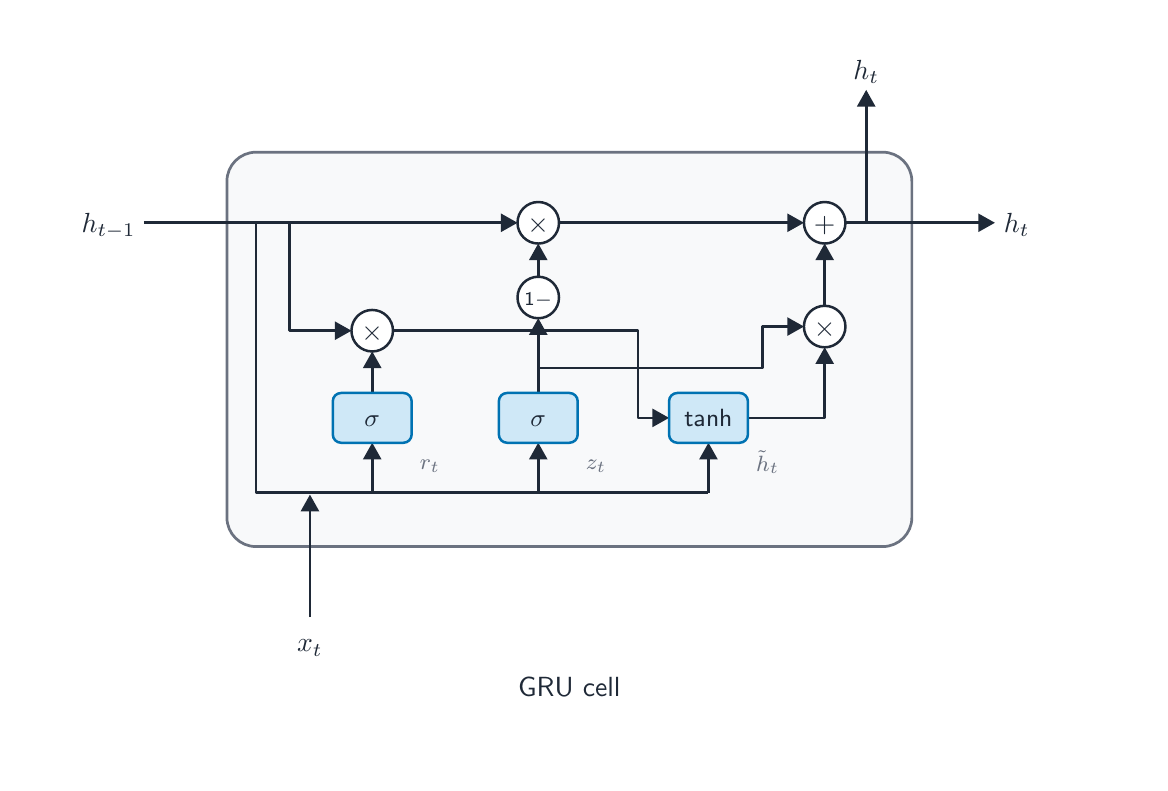
\begin{tikzpicture}[x=0.75pt, y=-0.75pt]
  \tikzset{
    xm cell-body 12vx01w/.style={fill=xm2, draw=xm3, line width=0.98pt, rounded corners=10.5pt},
    xm flow 1yp2gsv/.style={draw=xm4, line width=1.05pt},
    xm flow 7njxta/.style={fill=xm4, line join=round},
    xm wire 1djkw30/.style={draw=xm4, line width=0.95pt, line join=round},
    xm flow 1y86laf/.style={draw=xm4, line width=0.95pt},
    xm flow 1djkw30/.style={draw=xm4, line width=0.95pt, line join=round},
    xm op 16xaacs/.style={fill=xm1, draw=xm4, line width=0.9pt},
    xm text xm4/.style={text=xm4, inner sep=0},
    xm gate 17c83pb/.style={fill=xm5, draw=xm6, line width=0.9pt, rounded corners=3pt},
    xm text xm3/.style={text=xm3, inner sep=0},
  }
  \fill[xm1] (0,0) rectangle (536,354);
  % Diagram
  \path[xm cell-body 12vx01w] (96,60) rectangle ++(330,190);
  \path[xm flow 1yp2gsv] (56,94) -- (229,94);
  \path[xm flow 7njxta] (236,94) -- (228,98.5) -- (228,89.5) -- cycle;
  \path[xm flow 1yp2gsv] (256,94) -- (367,94);
  \path[xm flow 7njxta] (374,94) -- (366,98.5) -- (366,89.5) -- cycle;
  \path[xm flow 1yp2gsv] (394,94) -- (459,94);
  \path[xm flow 7njxta] (466,94) -- (458,98.5) -- (458,89.5) -- cycle;
  \path[xm wire 1djkw30] (110,94) -- (110,224) -- (328,224);
  \path[xm flow 1y86laf] (136,284) -- (136,232);
  \path[xm flow 7njxta] (136,225) -- (140.5,233) -- (131.5,233) -- cycle;
  \path[xm flow 1y86laf] (166,224) -- (166,207);
  \path[xm flow 7njxta] (166,200) -- (170.5,208) -- (161.5,208) -- cycle;
  \path[xm flow 1y86laf] (246,224) -- (246,207);
  \path[xm flow 7njxta] (246,200) -- (250.5,208) -- (241.5,208) -- cycle;
  \path[xm flow 1y86laf] (328,224) -- (328,207);
  \path[xm flow 7njxta] (328,200) -- (332.5,208) -- (323.5,208) -- cycle;
  \path[xm flow 1y86laf] (166,176) -- (166,163);
  \path[xm flow 7njxta] (166,156) -- (170.5,164) -- (161.5,164) -- cycle;
  \path[xm flow 1djkw30] (126,94) -- (126,146) -- (149,146);
  \path[xm flow 7njxta] (156,146) -- (148,150.5) -- (148,141.5) -- cycle;
  \path[xm flow 1djkw30] (176,146) -- (294,146) -- (294,188) -- (302,188);
  \path[xm flow 7njxta] (309,188) -- (301,192.5) -- (301,183.5) -- cycle;
  \path[xm flow 1y86laf] (246,176) -- (246,147);
  \path[xm flow 7njxta] (246,140) -- (250.5,148) -- (241.5,148) -- cycle;
  \path[xm flow 1y86laf] (246,120) -- (246,111);
  \path[xm flow 7njxta] (246,104) -- (250.5,112) -- (241.5,112) -- cycle;
  \path[xm flow 1djkw30] (246,164) -- (354,164) -- (354,144) -- (367,144);
  \path[xm flow 7njxta] (374,144) -- (366,148.5) -- (366,139.5) -- cycle;
  \path[xm flow 1djkw30] (347,188) -- (384,188) -- (384,161);
  \path[xm flow 7njxta] (384,154) -- (388.5,162) -- (379.5,162) -- cycle;
  \path[xm flow 1y86laf] (384,134) -- (384,111);
  \path[xm flow 7njxta] (384,104) -- (388.5,112) -- (379.5,112) -- cycle;
  \path[xm flow 1yp2gsv] (404,94) -- (404,37);
  \path[xm flow 7njxta] (404,30) -- (408.5,38) -- (399.5,38) -- cycle;
  \path[xm op 16xaacs] (246,94) circle[radius=10];
  \node[xm text xm4, font=\sffamily\fontsize{9.75}{11.7}\selectfont, anchor=base] at (246,98.73) {\ensuremath{\times}};
  \path[xm op 16xaacs] (384,94) circle[radius=10];
  \node[xm text xm4, font=\sffamily\fontsize{9.75}{11.7}\selectfont, anchor=base] at (384,98.73) {+};
  \path[xm op 16xaacs] (384,144) circle[radius=10];
  \node[xm text xm4, font=\sffamily\fontsize{9.75}{11.7}\selectfont, anchor=base] at (384,148.73) {\ensuremath{\times}};
  \path[xm op 16xaacs] (246,130) circle[radius=10];
  \node[xm text xm4, font=\sffamily\fontsize{7.5}{9}\selectfont, anchor=base] at (246,133.64) {1\ensuremath{-}};
  \path[xm op 16xaacs] (166,146) circle[radius=10];
  \node[xm text xm4, font=\sffamily\fontsize{9.75}{11.7}\selectfont, anchor=base] at (166,150.73) {\ensuremath{\times}};
  \path[xm gate 17c83pb] (147,176) rectangle ++(38,24);
  \node[xm text xm4, font=\sffamily\fontsize{9}{10.8}\selectfont, anchor=base] at (166,192.37) {\ensuremath{\sigma}};
  \path[xm gate 17c83pb] (227,176) rectangle ++(38,24);
  \node[xm text xm4, font=\sffamily\fontsize{9}{10.8}\selectfont, anchor=base] at (246,192.37) {\ensuremath{\sigma}};
  \path[xm gate 17c83pb] (309,176) rectangle ++(38,24);
  \node[xm text xm4, font=\sffamily\fontsize{9}{10.8}\selectfont, anchor=base] at (328,192.37) {tanh};
  \node[xm text xm4, font=\sffamily\fontsize{9.75}{11.7}\selectfont, anchor=base] at (39,98.73) {$h_{t-1}$};
  \node[xm text xm4, font=\sffamily\fontsize{9.75}{11.7}\selectfont, anchor=base] at (476.54,98.73) {$h_t$};
  \node[xm text xm4, font=\sffamily\fontsize{9.75}{11.7}\selectfont, anchor=base] at (136,300.73) {$x_t$};
  \node[xm text xm4, font=\sffamily\fontsize{9.75}{11.7}\selectfont, anchor=base] at (404,24.73) {$h_t$};
  \node[xm text xm3, font=\sffamily\fontsize{8.25}{9.9}\selectfont, anchor=base] at (193.78,213) {$r_t$};
  \node[xm text xm3, font=\sffamily\fontsize{8.25}{9.9}\selectfont, anchor=base] at (273.86,213) {$z_t$};
  \node[xm text xm3, font=\sffamily\fontsize{8.25}{9.9}\selectfont, anchor=base] at (356.53,213.7) {$\tilde{h}_t$};
  \node[xm text xm4, font=\sffamily\fontsize{9.75}{11.7}\selectfont, anchor=base] at (261,322) {GRU cell};
\end{tikzpicture}
\end{document}
